% begin module trig-functions-example2
\begin{frame}
\begin{example}
If $\cos \theta = \frac{2}{5}$ and $0 < \theta < \frac{\pi}{2} $, find the other five trigonometric functions of $\theta$.
\begin{columns}[c]
\column{.3\textwidth}

\psset{xunit=1cm,yunit=1cm}
\begin{pspicture}(-0.1,-0.5)(4,5.1)
\fcBoundingBox{-0.1}{-0.5}{4}{5.1}
\uncover<2->{
\rput[l](2,2.6){ $ \alertNoH{4,5}{x=} \fcAnswerUncover{1}{5}{\alertNoH{7,9,11,15} {\sqrt{21}}} $}
\rput[br](0.95,2.5){ \alertNoH{7,11,13}{$5$}}
\rput[t](1, -0.1){\alertNoH{9,13, 15}{$2$}}
}
\psline(0,0)(2,0)(2,5)(0,0)
\psline(1.8,0)(1.8,0.2)(2,0.2)
\psarc[linecolor=red](0,0){0.3}{0}{68.19859}
\rput(0.4,0.3){$\theta$}
\end{pspicture}
%\column{.3\textwidth}
%\ \only<handout:0| -1>{%
%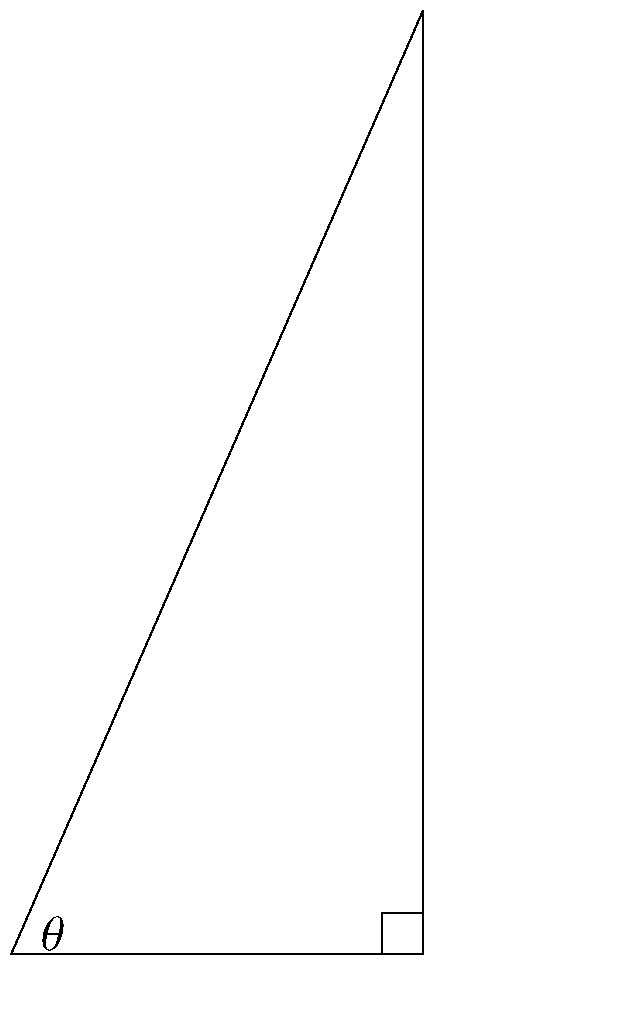
\includegraphics[height=6cm]{trigonometry/pictures/app-d-ex4a.pdf}%
%}%
%\only<handout:0| 2-3>{%
%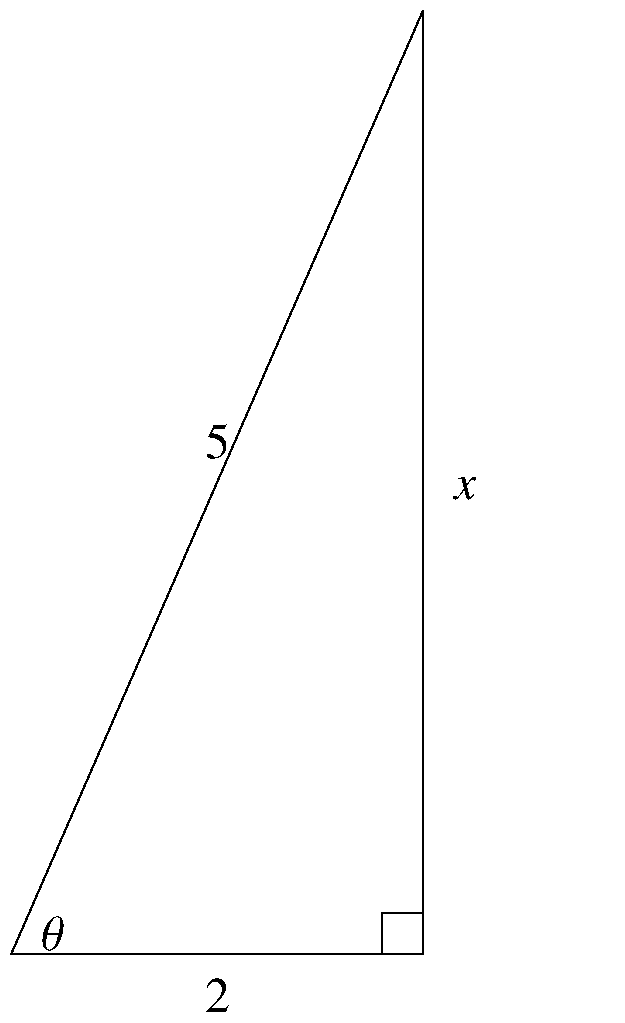
\includegraphics[height=6cm]{trigonometry/pictures/app-d-ex4b.pdf}%
%}%
%\only<4->{%
%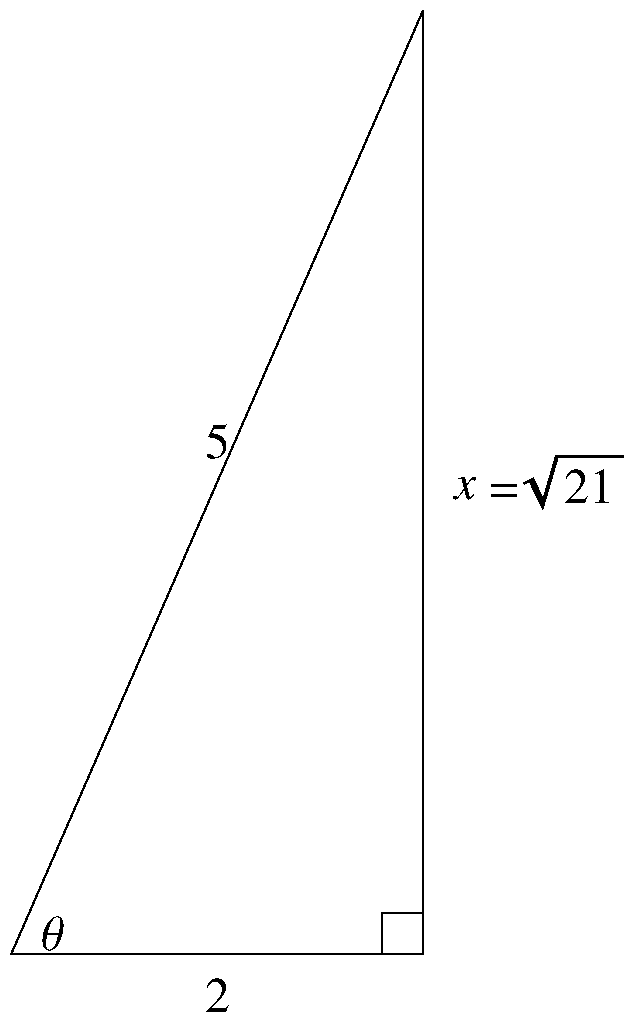
\includegraphics[height=6cm]{trigonometry/pictures/app-d-ex4c.pdf}%
%}%
\column{.7\textwidth}
\begin{itemize}
\item<2->  Label the hypotenuse with length 5 and the adjacent side with length 2.
\item<3->  Pythagorean theorem: $x^2 +2^2 = 5^2$.
\item<4->  Therefore $x^2 = \fcAnswer{5}{21}$, so $x = \fcAnswer{5}{\sqrt{21}}$.
\end{itemize}
\[
\begin{array}{cc}
\alert<handout:0| 6-7>{%
\sin \theta = %
\fcAnswer{7}{%
\frac{\sqrt{21}}{5}%
}}&%
\alert<handout:0| 8-9>{%
\tan \theta = %
\fcAnswer{9}{%
\frac{\sqrt{21}}{2}%
}}\\%
& \\
\alert<handout:0| 10-11>{%
\csc \theta = %
\fcAnswer{11}{%
\frac{5}{\sqrt{21}}%
}}&%
\alert<handout:0| 12-13>{%
\sec \theta = %
\fcAnswer{13}{%
\frac{5}{2}%
}}\\%
& \\
\alert<handout:0| 14-15>{%
\cot \theta = %
\fcAnswer{15}{%
\frac{2}{\sqrt{21}}%
}}&%
\end{array}
\]
\end{columns}
\end{example}
\end{frame}
% end module trig-functions-example2
